\chapter{Introduction to NoSQL Injection}
This section outlines the concept of NoSQL injection and how it derives from conventional SQL injection. A definition of NoSQL injection is given along with a detailed analysis of the corresponding attacker models.

\section{From SQL to NoSQL Injection}
\label{sec:fromSQLtoNoSQLinjection}
Injection attacks on relational databases represent the major web application vulnerability of the last decade. Thereby, the three tier architecture composed of client, server and database plays an important role. Since data obtained from the client can be arbitrary manipulated, input validation and sanitizing represent important principles for the the server-side. Otherwise, unvalidated input may find its way into sensitive operations, that cause injection vulnerabilities. In case unvalidated data is used to build database queries, an attacker is able to alter the SQL statement's structure. Suchlike vulnerabilities represent serious threats, especially due to the direct data access in combination with the Touring completeness of the injected SQL context.\\ 

This situation changed with the emerging generation of NoSQL databases. A variety of new query techniques was introduced next to SQL. For many databases, JSON-based or parameterized function calls replaced the conventional SQL approach. These simplified methods lead to a more straightforward database access and enabled unstructured data models. All the same, program logic moved from the database to the application layer due to functional limitations of the queries. Complex operations, such as data constraints or checks, that were previously executed directly on the database with SQL, have to be implemented within the application layer. Bypassing these logical constraints in order to achieve a certain database behavior constitutes an important aspect in the context of NoSQL injection. \\ 

Beside the query techniques, also the architecture of systems diversified with the emerged NoSQL databases. Relational databases are similar regarding their strengths and weaknesses, leading to a deployment in typical system structures, like the three tier model. In contrast to that, NoSQL databases discern in their focused area of application. Special requirements demand for tailored databases or even a combination of them. This leads to heterogeneous system landscapes deploying different databases and technology stacks for distinct purposes. Data exchange between multiple databases becomes an vital aspect that has to be managed. The resulting diversity of system designs as well as the data exchange between different data models has to be considered for the attack surface of NoSQL injection. All in all, NoSQL injection faces a much more diverse environment in contrast to conventional SQL injection.

\section{Definition of NoSQL Injection}

In order to give a definition for injection attacks against NoSQL databases, multiple aspects have to be taken into account. The objective of an attack has to be clarified as well as the mightiness of an attacker. In the course of this, the varying system structures has to be considered. Thus, attacker models for NoSQL injection expose themselves much more diverse in comparison to conventional SQL injection. In general, NoSQL injection can be defined the following way:\\

\begin{description}
\item [NoSQL Injection] represents a class of attacks against non-relational databases, that cause unintended behavior of a query through insertion of malicious data into the query context. These vulnerabilities originate from unvalidated user input used as or as a part of a database query. Depending on the attacked database, the injected input is crafted with the aim to trigger unintended operations of the database layer affecting confidentiality, integrity or availability of data.
\end{description}

Similar to other classes of attacks, NoSQL injection is directed against at least one of the three security goals - confidentiality, integrity and availability. This class of attack is focused on the database layer of an application or more precisely the therein stored data. The attacker goal of NoSQL injection is to compromise this data with regard to any of the mentioned security goals. Unauthorized modification or retrieval of data as well as restriction of data access for others, represent successful attacks. These results can be achieved by triggering malicious query behavior, especially with regard to typical create, read, update and delete operations. Malicious behavior can be accomplished through manipulation of existing queries as well as the invocation of unauthorized queries. Bypasses for preceding confidentiality and integrity checks allow such query manipulation and invocation and constitute an important aspect for this class of attacks. User provided input in turn enables users as well as attackers to influence database queries. When data received from user input is not properly sanitized for the query context, an attacker might be able to manipulate the semantics and structure of the database operation. Inputs provided by users derive from requests received from clients. Since their content can be manipulated, these requests represent the attacker surface for NoSQL injection. Arbitrary manipulation is only limited by the fixed protocol structure used for the request. Otherwise, further processing of the request on the recipient side may fail. For an attack, a request with adapted contents is built, that leads to a database query with malicious user input. The database interprets the triggered query in a way that breaks one of the security goals for the underlying data. These circumstances define a successful NoSQL injection attack.\\

The given definition of NoSQL injection is described in a relatively generic way. This goes in accordance with the in section \ref{sec:fromSQLtoNoSQLinjection} elucidated diverse system environments. On account of these circumstances, the way user input takes until it reaches the database query distinguishes depending on the system environment. Therefore, the phase between attacker initiated request and actual invocation of a database operation faces different scenarios. To address this in scope of the NoSQL injection definition, the following sections analyze the most significant scenarios and outline the according attacker models.

\subsection{Common Attacker Model}

% known attacker model similar to SQL injection
% three tier model common in web context
% ATTACKER Mightiness + GOAL

\begin{figure}[h]
\centering
  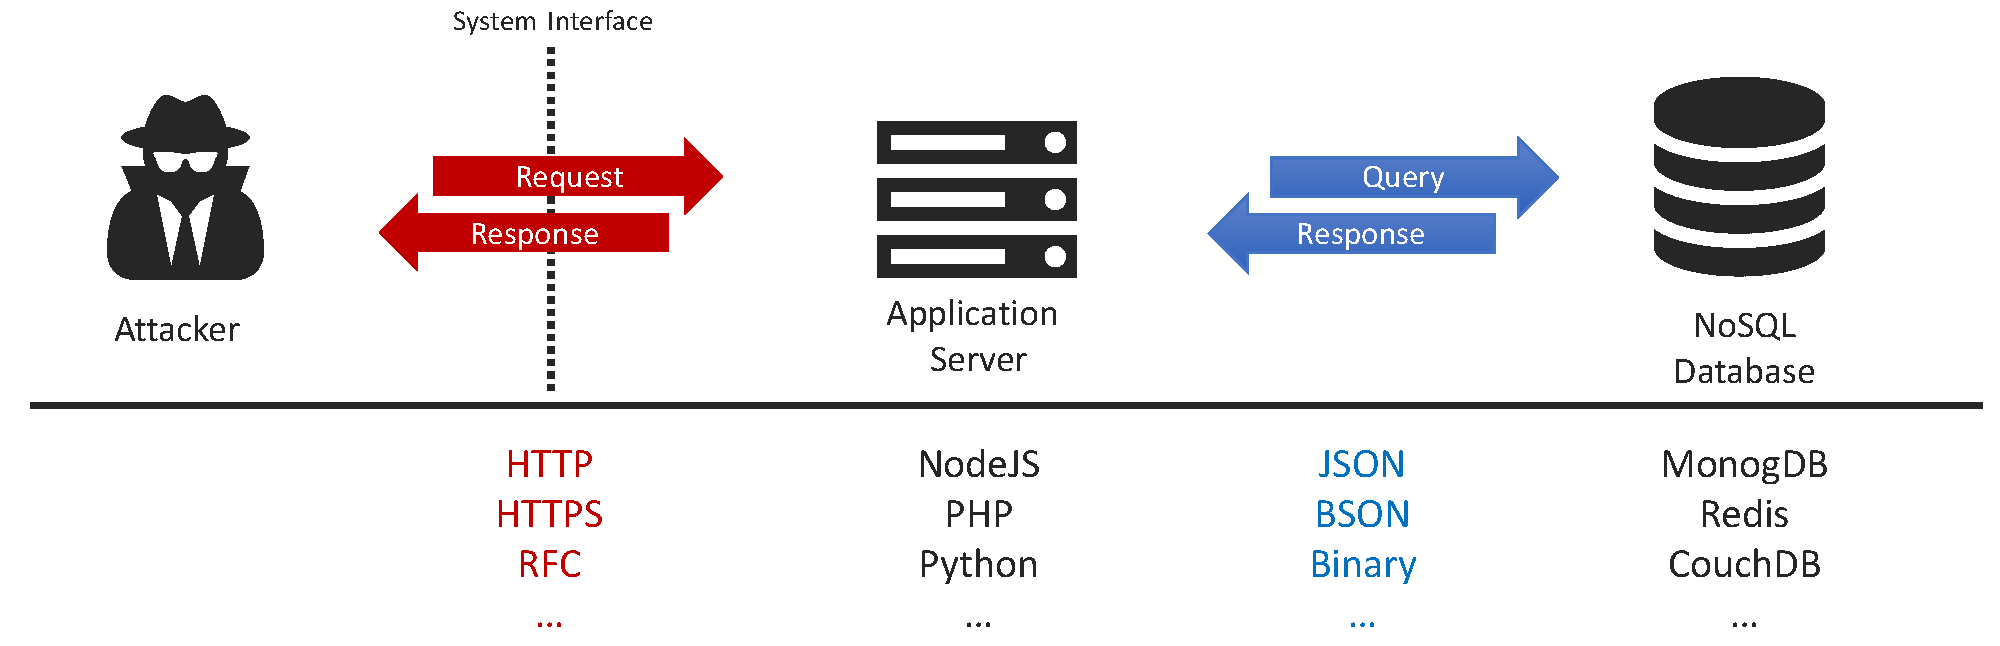
\includegraphics[width=1\linewidth]{Images/attacker_model_normal}
  \caption{Common attacker model for NoSQL injection}
  \label{fig:normalAttackerModel}
\end{figure}

% Objective

\subsection{Extended Attacker Model}

% complex system architecture
% multiple systems for different purposes
% data exchange with different formats
% normal entry in one database, critical entry in another
% 2-step approach
% assumption to be able to insert arbitrary data into a external system or further 
% attacker is able to insert arbitrary entry in database
% ATTACKER Mightiness + GOAL (- insert)

\begin{figure}[h]
\centering
  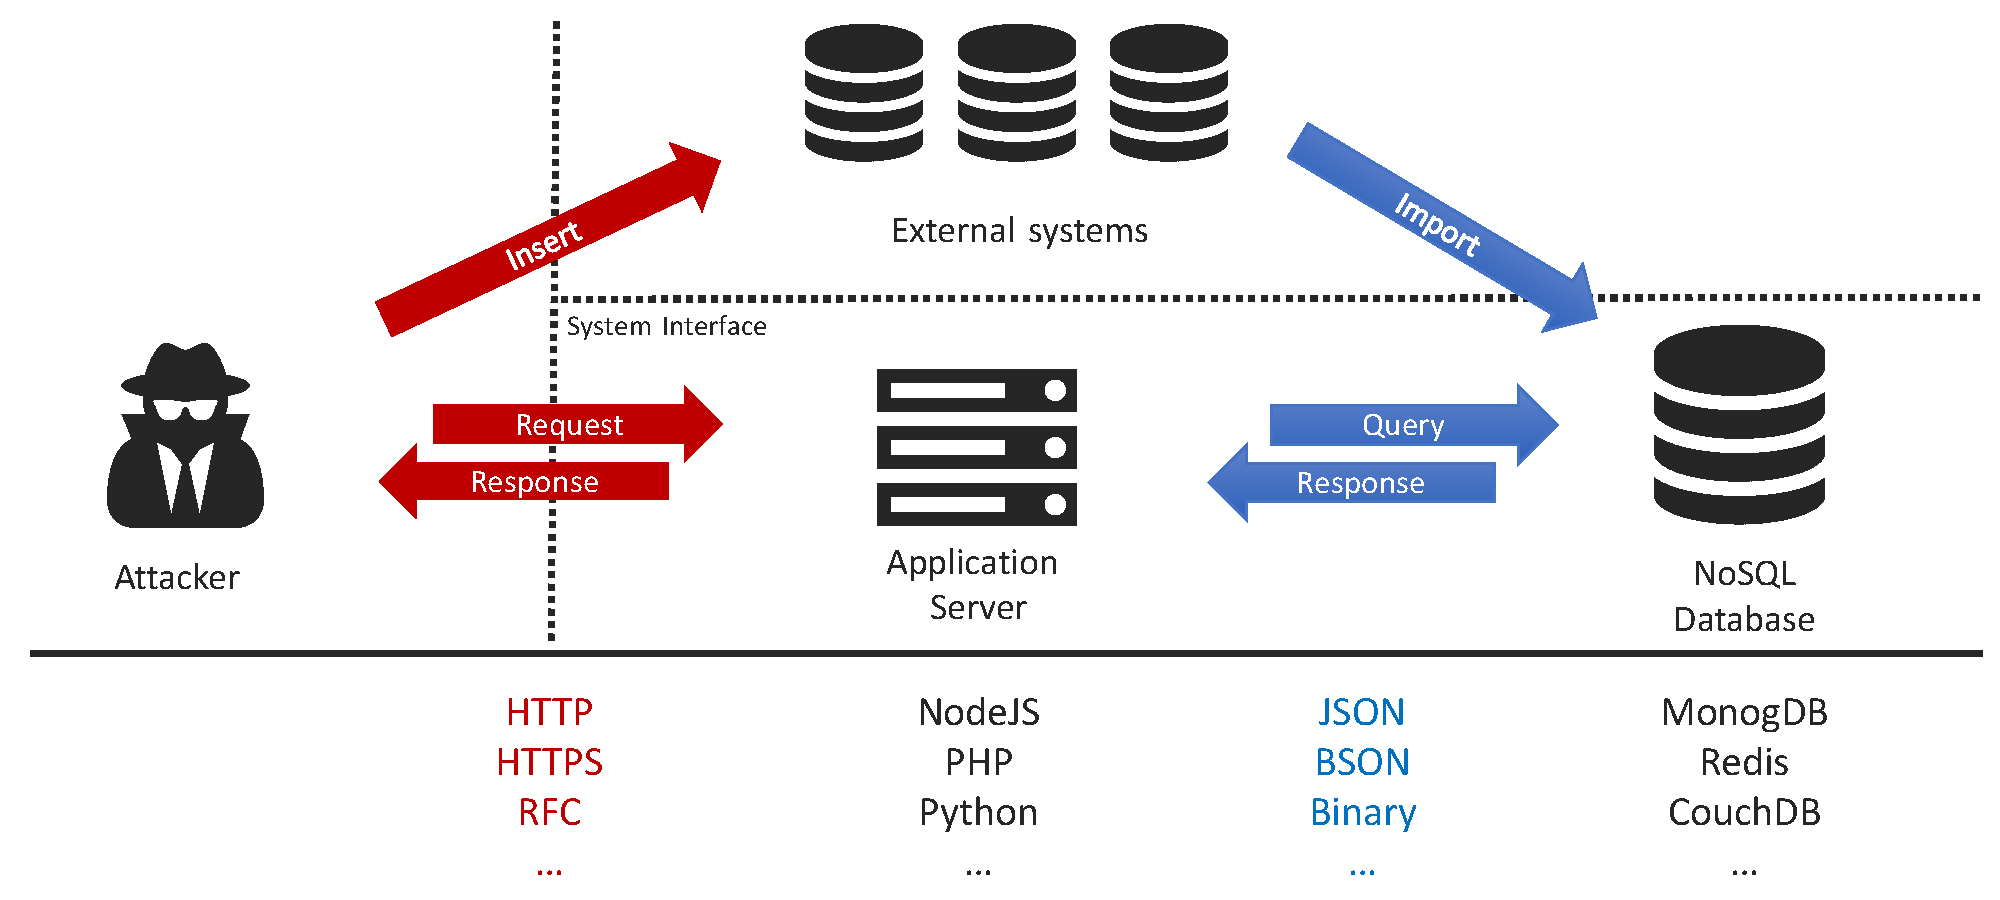
\includegraphics[width=1\linewidth]{Images/attacker_model_extended}
  \caption{Extended attacker model for NoSQL injection}
  \label{fig:extendedAttackerModel}
\end{figure}

% Objective

\subsection{Direct Attacker Model}

The deployment of RESTful interfaces allows a direct access from the client, omitting any application layer. Databases such as CouchDB explicitly refer to this architectural style for a simpler application design.

% RESTful interface 
% direct access from client - no application layer needed
% normal application uses only read
% but write other operations can be injected
% different attacker surface! direct REST access via HTTP (parameter in URL or Body)
% ATTACKER Mightiness + GOAL

\begin{figure}[h]
\centering
  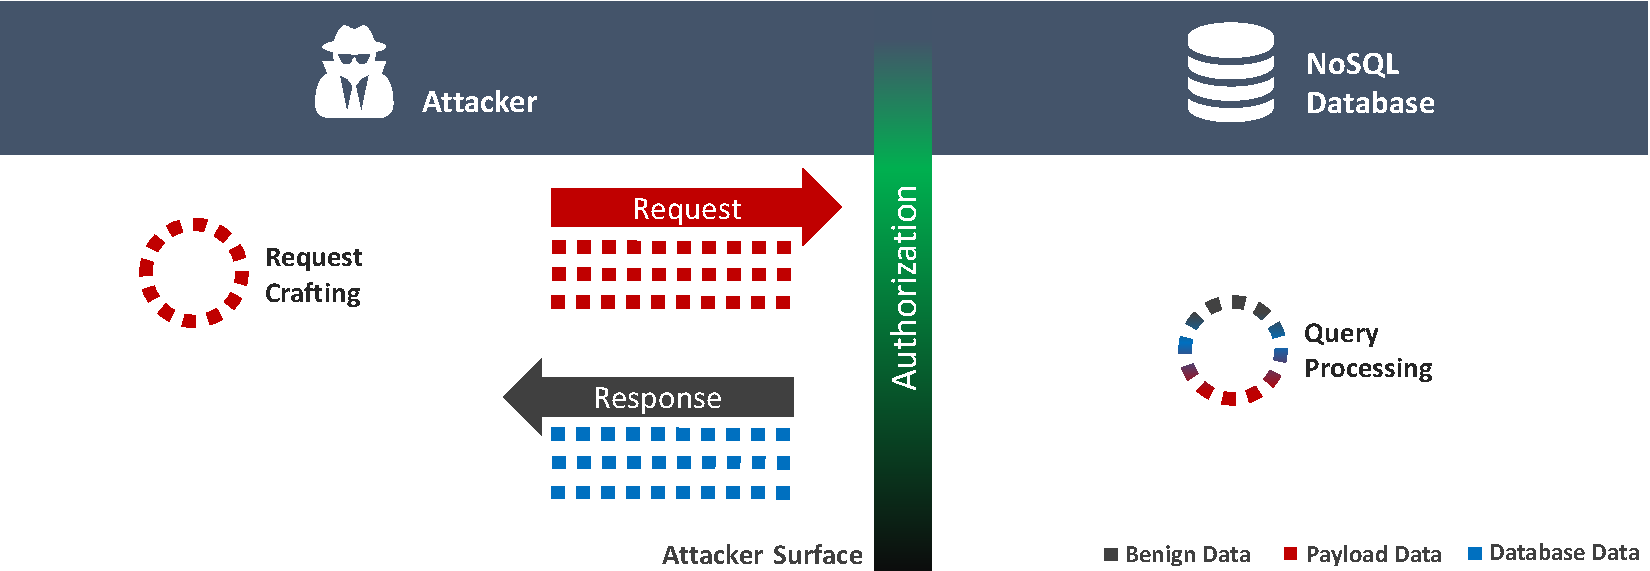
\includegraphics[width=1\linewidth]{Images/attacker_model_direct}
  \caption{Direct attacker model for NoSQL injection}
  \label{fig:extendedAttackerModel}
\end{figure}

% Objective 1 covered with this section!


\section{Considered Technology Stack}

% focused on HTTP/HTTPS as attacker surface, but other protocols possible
% control over entire request, in case of HTTP HEADER + BODY and the HTTP-Method
% Which HTTP methods are relevant (CRUD)
% parameters for application server interesting, these usually are used for server-side processing
% Body (JSON, XML, x-www-form-urlencoded), Header (Cookies), URL (Querystring, Path)
% type of system architecture to attack
% ACTUAL definition 

% analyze the underlying problem of known and found injection attacks
\subsection{Selected Databases}
\subsection{Selected Application Platforms}
\subsection{Selected Application Layer Protocols}

\textbf{HTTP}
\textbf{HTTPS}